\documentclass[conference]{IEEEtran}
\IEEEoverridecommandlockouts
% 1. change the format of refernence
\renewcommand{\thesection}{\arabic{section}}
\renewcommand{\thesubsection}{\thesection.\arabic{subsection}}
\renewcommand{\thesubsubsection}{\thesubsection.\arabic{subsubsection}}

% 2. Change the actual numbering format displayed in the title (针对 IEEEtran 模板的强制覆盖)
\renewcommand{\thesectiondis}{\thesection.}
\renewcommand{\thesubsectiondis}{\thesubsection.}
\renewcommand{\thesubsubsectiondis}{\thesubsubsection.}

% The preceding line is only needed to identify funding in the first footnote. If that is unneeded, please comment it out.
\usepackage{cite}
\usepackage{wasysym}
\usepackage{amsmath,amssymb,amsfonts}
\usepackage{algorithmic}
\usepackage{cuted}
\usepackage{graphicx}
\usepackage{xcolor}
\usepackage{newtxtext}
\usepackage{natbib}
\usepackage{float}
\usepackage{siunitx}
\usepackage{booktabs}
\usepackage{newtxmath}
% ── Utility commands ──────────────────────────────────────
\newcommand{\UAV}{\textsc{SolarWing-V}}          % project codename
\newcommand{\degrees}{$^{\circ}$}

\graphicspath{{Figure/}}

\def\BibTeX{{\rm B\kern-.05em{\sc i\kern-.025em b}\kern-.08em
    T\kern-.1667em\lower.7ex\hbox{E}\kern-.125emX}}
\begin{document}

\title{Solar-Assisted Tilt-Rotor UAV for Low-Altitude Logistics\\
{\footnotesize \textsuperscript{*}Project in Design for Manufacturing (034371)}
}

\author{
\IEEEauthorblockN{Zhuorui Yun,\ Youwen Han,\ Wulin Xi,\ Xinlei Lin,\ Rui Zhong}
\IEEEauthorblockA{
\textit{Mechanical Engineering and Robotics,
Guangdong Technion -- Israel Institute of Technology}, Shantou, China\\
\{yun24239, han24588, xi24277, lin24872, zhong24349\}@gtiit.edu.cn
}
}

\maketitle

\begin{abstract}
With the acceleration of global urbanization, traditional ground transportation struggles to meet the growing demand for urban last-mile logistics and express delivery. This paper proposes a design scheme for a tilt-rotor solar Unmanned Aerial Vehicle (UAV) based on a Vertical Take-Off and Landing (VTOL) architecture, aiming to provide a faster, more efficient, and environmentally friendly transportation method for urban environments. This scheme combines the precise hovering and VTOL capabilities of multi-rotor UAVs with the high-speed, long-endurance advantages of fixed-wing UAVs. Furthermore, flexible solar cell arrays are integrated into the wing surfaces to significantly extend flight endurance. In this study, SolidWorks was used for the 3D full-machine modeling and tilt-mechanism design; subsequently, ANSYS software was utilized for Computational Fluid Dynamics (CFD) simulation and Finite Element Analysis (FEA) for structural statics. The simulation results verify the aerodynamic stability during the tilt transition phase and the structural reliability of key load-bearing components. This research provides a viable hardware design reference for the next-generation urban green aviation logistics system.
\end{abstract}

\begin{IEEEkeywords}
VTOL UAV, solar-powered drone, tilt-rotor, urban air mobility, last-mile delivery, CFD, FEA, SolidWorks, ANSYS.
\end{IEEEkeywords}

\section{Introduction}

\subsection{Background and context}
The exponential growth of e-commerce, combined with increasing urban congestion, has created significant pressure on traditional ground-based delivery infrastructure. Urban centers worldwide face the dual challenge of meeting growing logistics demands while simultaneously reducing traffic congestion and carbon emissions. Unmanned aerial vehicles (UAVs), commonly referred to as drones, have emerged as a promising alternative delivery mechanism capable of bypassing surface-level bottlenecks (Stolaroff et al., 2018)\cite{b6}.

However, conventional UAV designs present fundamental trade-offs. Multirotor platforms offer vertical take-off capability but suffer from limited range and high power consumption due to continuous rotor thrust for lift. Fixed-wing designs provide aerodynamic efficiency at cruise but require runway infrastructure incompatible with dense urban environments. VTOL aircraft combining tilt-rotor mechanisms with fixed-wing aerodynamics represent a compelling middle ground, enabling both hover capability and efficient cruise flight (Saeed et al., 2018)\cite{b5}.

The integration of solar energy harvesting into UAV platforms further addresses the endurance limitation, allowing photovoltaic (PV) panels embedded in the wing surface to supplement or replace battery capacity during daytime operations \cite{b9}. The confluence of VTOL capability, solar energy harvesting, and advances in lightweight composite materials presents an opportunity to develop a practical urban logistics UAV.

\subsection{Existing Challenges and Motivation}
Currently, UAVs used for logistics are mainly divided into two categories: multi-rotor and fixed-wing. Multi-rotor UAVs (like quadcopters) offer flexible take-off and landing and stable hovering, making them suitable for narrow urban spaces, but they are limited by battery density, resulting in short flight times and small operational radii. Fixed-wing UAVs have long ranges and high speeds, but require runways or catapults, making them incapable of free take-off and landing among complex urban high-rises. In addition, frequent charging requirements reduce the operational efficiency of UAV fleets.

\subsection{Project Objectives}
Our aims are:
\begin{itemize}
    \item Design a VTOL UAV airframe with integrated tilt-rotor propulsion using SolidWorks software.
    \item Conduct aerodynamic and structural simulations using ANSYS CFD and FEA modules to evaluate performance under representative urban operating conditions.
    \item Analyze the feasibility of solar energy integration to extend flight endurance beyond battery-only limitations.
    \item Assess the suitability of the proposed system for urban last-mile delivery applications. 
\end{itemize}

\subsection{Scope and Delimitation}
This study is limited to simulation-based analysis; physical prototyping and flight testing are identified as future work. The urban environment is modeled as a representative mid-density city with average solar irradiance conditions corresponding to subtropical latitudes. Regulatory frameworks for urban UAV operations are discussed qualitatively but are not the primary focus of this paper.

\section{Literature Review}
All the technologies in our designed aircraft have undergone thorough feasibility verification. Please note sections \ref{AA}--\ref{SAUA} below for more information on 
technical details.

\subsection{Tilt-Rotor VTOL Technology}\label{AA}
TVTOL UAVs have been studied extensively across military, commercial, and research applications. Saeed et al. (2018) provide a comprehensive taxonomy of VTOL configurations, categorizing them into tilt-rotor, tilt-wing, tail-sitter, and hybrid lift-plus-cruise designs \cite{b5}. The tilt-rotor configuration, popularized by full-scale aircraft such as the V-22 Osprey, enables efficient transition between hover and forward flight by rotating nacelles housing both rotors and motors along a longitudinal axis.

For UAV-scale tilt-rotor systems, Flores et al. (2012) demonstrated stable autonomous transition control using a nonlinear control law, while Muraoka et al. (2009) validated aerodynamic performance of a quad tilt-rotor configuration through wind tunnel experiments \cite{b1}. These studies establish that tilt-rotor UAVs can achieve stable transition flight but require sophisticated control architectures, particularly during the conversion phase where rotor wake interacts with wing surfaces.


\subsection{Solar UAV Applications}
As a clean energy source, solar energy has been widely used in High-Altitude Long-Endurance (HALE) UAVs (such as the Zephyr project). Li et al. \cite{b2} showed that in low-altitude urban airspace, by optimizing the MPPT (Maximum Power Point Tracking) algorithm for thin-film solar cells, the effective endurance of fixed-wing UAVs can be increased by 25\% to 40\%. However, research combining solar technology with VTOL tilt architecture for high-frequency urban logistics delivery remains relatively scarce.

\subsection{Urban Logistics Delivery Demands}
According to the route planning research for urban UAV logistics by Wang and Chen \cite{b3}, an ideal urban delivery UAV needs an operational radius of at least 15 kilometers and a payload of over 5 kilograms, while also possessing extremely high crosswind resistance to cope with the urban ``canyon effect.''

\subsection{Structural Analysis of UAV Airframes}\label{SAUA}

Composite materials, particularly carbon fiber reinforced polymer (CFRP) and glass fiber reinforced polymer (GFRP), dominate modern UAV structural design due to their high specific strength and stiffness (Gundlach, 2012) \cite{b7}. FEA using tools such as ANSYS Mechanical has been widely applied to validate UAV structural integrity under aerodynamic and inertial loads. Brincker and Ventura (2015) provide foundational guidance on applying FEA to thin-shell aerospace structures, which is directly applicable to the wing and fuselage panels of the proposed design \cite{b8}.

\section{Methods}
\subsection{Design Overview}
The proposed UAV follows a fixed-wing airframe with a high-wing monoplane configuration, chosen to maximize upper-surface area available for solar panel integration. Four tilt-rotor nacelles are mounted in a quad configuration — two on the main wing and two on the rear stabilizer — enabling differential thrust for pitch, roll, and yaw control in hover mode, while all four rotors transition to forward-thrust orientation during cruise flight.
Key design parameters were established through preliminary sizing analysis based on target mission requirements: a delivery radius of 10 km, payload of up to 2 kg, and daytime-only operations with a minimum of 6 hours of solar availability. Table 1 summarizes the primary design specifications.

\begin{table}[htbp]
\centering
\caption{Primary Design Specifications}
\label{tab:specs}
\renewcommand{\arraystretch}{1.3}
\begin{tabular}{lll}
\toprule
\textbf{Parameter} & \textbf{Value} & \textbf{Remarks} \\
\midrule
Wingspan              & \SI{3.05}{m}     & Constrained by urban landing zone \\
Wing Area             & $\approx$\SI{1.15}{m^2}  & Aspect ratio $\approx$8.1 \\
MTOW                  & \SI{12.0}{kg}    & Including 5\,kg payload \\
Payload Capacity      & \SI{5.0}{kg}     & Two SF Express F3 containers \\
Cruise Speed          & \SI{65}{km/h}    & Design point \\
Hover Power           & $\approx$\SI{1500}{W}    & 12S high-torque propulsion \\
Solar Panel Area      & \SI{0.95}{m^2}   & Upper wing surface, IBC cells \\
Solar Panel Efficiency& \SI{24.5}{\%}    & Flexible IBC, commercial grade \\
Battery Capacity      & \SI{22000}{mAh}  & 44.4\,V (12S), Si-anode solid-state Li-ion \\
Battery Energy        & $\approx$\SI{977}{Wh}    & Gross; usable $\approx$880\,Wh \\
\bottomrule
\end{tabular}
\end{table}

\subsection{Configuration and CAD Modelling (SolidWorks)}
\subsubsection{Overall Configuration}

\begin{figure}[htbp]
  \centering
  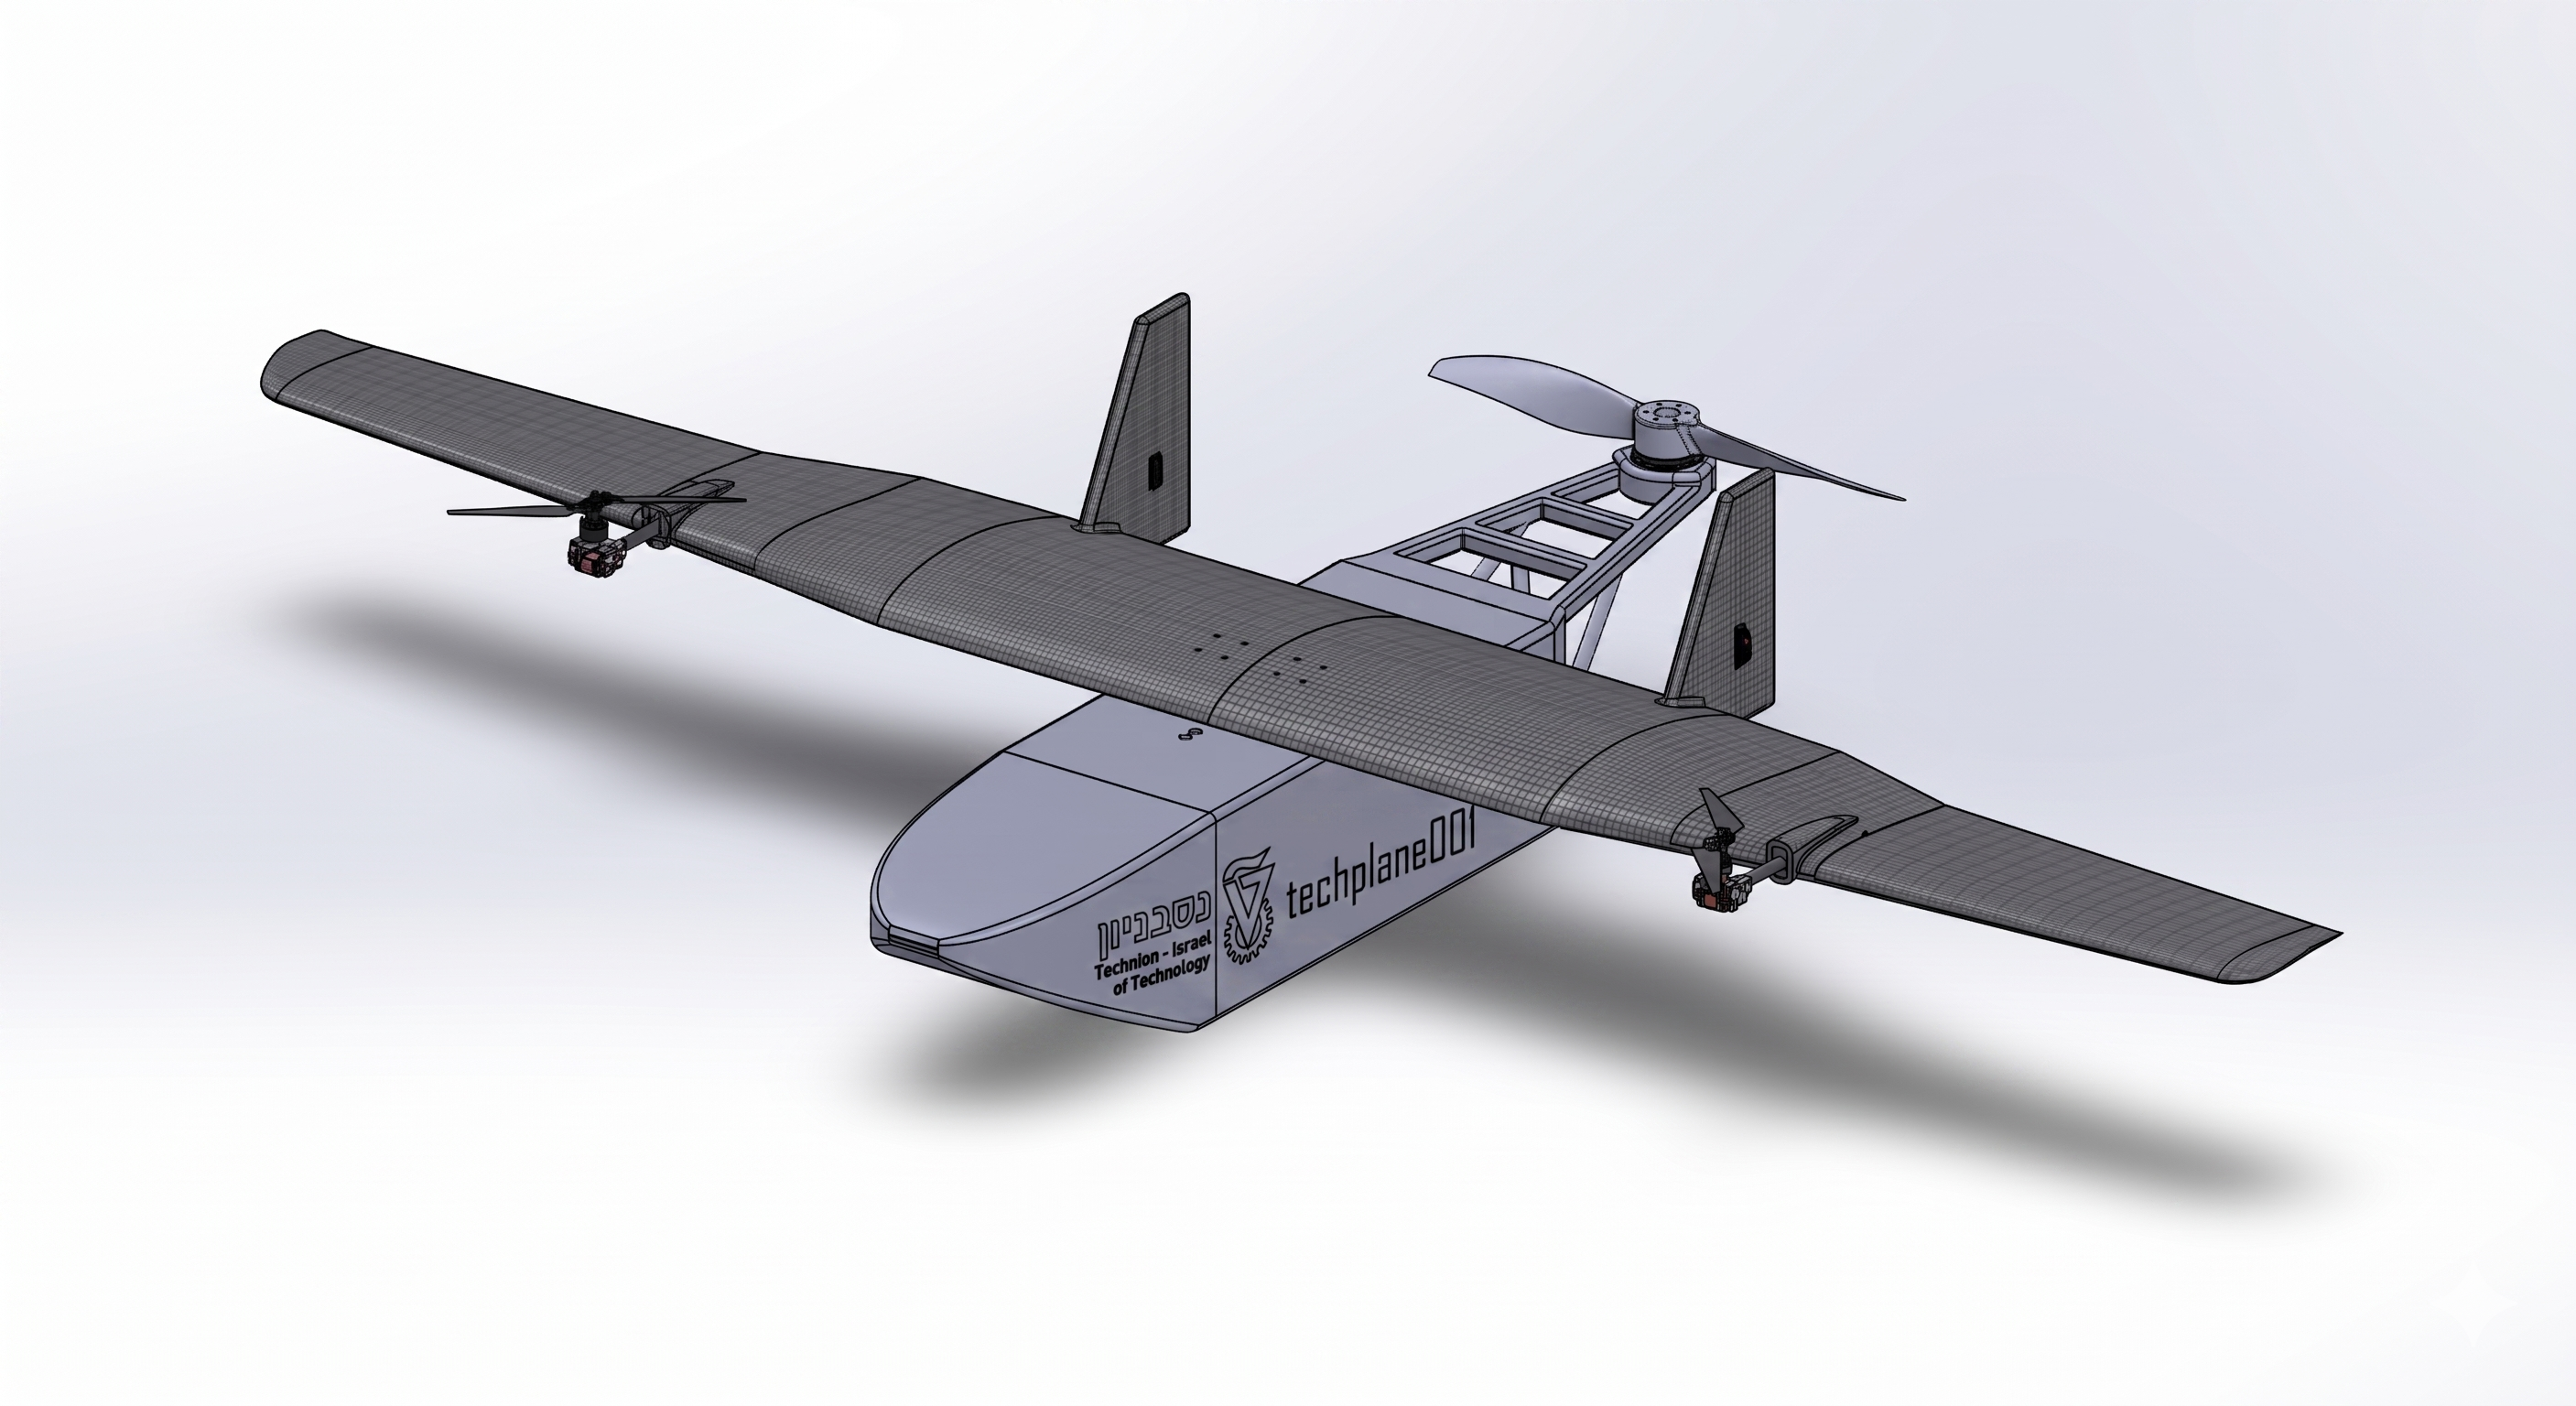
\includegraphics[width=\columnwidth]{three-view.png}
  \caption{Three-view orthographic drawing of the \UAV{} showing the
           high-wing monoplane configuration, twin-boom empennage,
           four tilt-rotor nacelles, and integrated solar panel array.}
  \label{fig:cad_overview}
\end{figure}

The \UAV{} adopts a conventional mid-wing, twin-boom pusher–tractor
tilt-rotor layout.
Two large-diameter (approximately \SI{0.50}{m}) tractor rotors are mounted on
tilting nacelles at the wingtips, providing both hover thrust and forward cruise
thrust after \SI{90}{\degree} rotation.
A pair of smaller (\SI{0.25}{m}) fixed-pitch elevon motors at the twin-boom
empennage provide pitch and hover-roll authority during transition.
The central fuselage is a semi-monocoque composite shell housing the avionics bay,
battery compartment, and a ventral cargo door for the F3 containers.

\subsubsection{Wing Design}

The wing is a one-piece composite structure with a NACA 4415 aerofoil section,
chosen for its benign stall characteristics and high maximum lift coefficient
(\(C_{L,\max} \approx 1.52\)).
A tapered planform (\(\lambda = 0.6\)) reduces induced drag, with washout of
\SI{2}{\degree} to ensure tip stall is preceded by root stall.
The primary spar is a pultruded carbon-fibre tube (\diameter 25\,mm $\times$ 2\,mm wall),
with a secondary rear spar (\diameter 12\,mm) supporting the trailing-edge elevon servos.
Ribs are laser-cut 3-mm Depron foam with 0.5-mm carbon-fibre face sheets,
forming a semi-monocoque that bears torsion loads.

\subsubsection{Tilt Mechanism}

\begin{figure}[htbp]
  \centering
  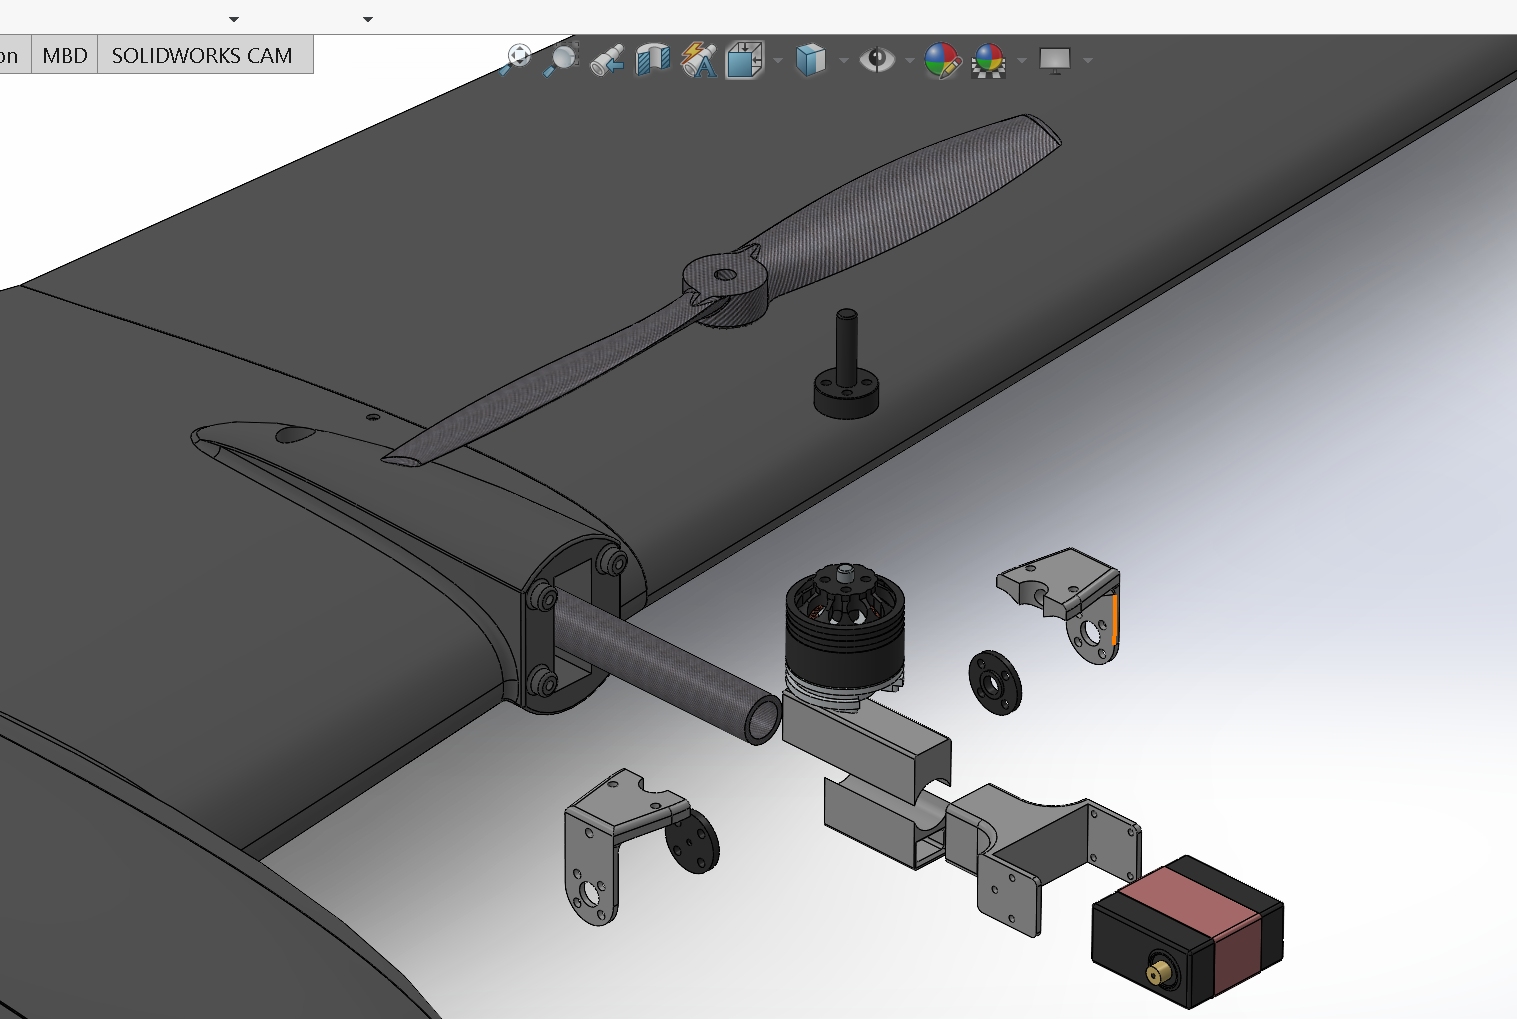
\includegraphics[width=\columnwidth]{tilting_explosion.png}
  \caption{Exploded assembly view of the tilt-rotor nacelle mechanism,
           illustrating the \SI{90}{\degree} rotation arc between hover
           (vertical thrust) and cruise (horizontal thrust) configurations,
           the dual-redundant servo actuator, geared drive, and detent latch.}
  \label{fig:tilt_mechanism}
\end{figure}

The wingtip nacelles rotate through a \SI{90}{\degree} arc via a dual-redundant
RC servo actuator driving a 6:1 geared mechanism.
A detent latch locks the nacelle at both extreme positions (hover: vertical thrust;
cruise: horizontal thrust), removing servo holding current and improving reliability.
The tilt axis is located at the aerodynamic centre of the nacelle to minimise
pitching moment change during transition.

\subsubsection{Photovoltaic Integration}

Flexible IBC PV modules (\SI{1.5}{mm} total thickness) are bonded to the upper
wing skin using a UV-resistant structural adhesive.
The module layout occupies the inboard 65\% of each wing panel,
yielding \SI{0.95}{m^2} of active PV area.
Electrical interconnection uses redundant series–parallel stringing to maximise
yield under partial shading caused by urban building obstructions,
with a maximum power point tracking (MPPT) converter achieving 97\% conversion efficiency.

\subsubsection{Payload Bay}

The cargo bay is dimensioned to accommodate two SF Express F3 logistics containers
(each \SI{300}{mm} $\times$ \SI{200}{mm} $\times$ \SI{160}{mm}, maximum gross mass \SI{2.5}{kg}).
A spring-loaded ventral door actuated by a single servo releases the payload via
a gravity-drop mechanism, enabling rapid sub-\SI{30}{s} delivery without landing.

\subsection{Aerodynamic Simulation — ANSYS Fluent (CFD)}
Computational fluid dynamics analysis was conducted using \textbf{\textit{ANSYS Fluent 2024 R1}}. The simulation domain was defined as a rectangular far-field region with dimensions $10L \times 6L \times 6L$ (where L = wingspan = 2.4 m), with the UAV positioned at the domain center. Boundary conditions were set as velocity-inlet (freestream), pressure-outlet, and no-slip wall on all UAV surfaces.
Two flight conditions were simulated: (1) hover mode at zero freestream velocity with rotating rotor disk boundary conditions (actuator disk model), and (2) cruise mode at 65 km/h at angles of attack ranging from $-4 ^\circ$ to $+12^\circ$ at $2^\circ$ increments. The $k-\omega$ SST turbulence model was selected for its accuracy in adverse pressure gradient flows relevant to wing stall prediction. The computational mesh comprised approximately 8.5 million polyhedral cells with boundary layer refinement on wing surfaces to achieve $y^+ <1$.

\subsection{Structural Analysis — ANSYS Mechanical (FEA)}
\label{sec:fea_method}

Finite element analysis was performed using \textbf{\textit{ANSYS Mechanical 2024 R1}} to evaluate the structural integrity of the wing assembly and tilt-nacelle mount bracket under representative load cases.

The wing structure was modelled as a shell/solid hybrid: the primary spar as a 3-D solid body meshed with quadratic tetrahedral elements (SOLID187), and the wing skin panels as shell elements (SHELL281) with composite layup definitions. The nacelle bracket was modelled as a solid aluminium 7075-T6 body. The global mesh size was \SI{5}{mm}, refined to \SI{1.5}{mm} at stress concentration zones (spar root, bracket bolt holes). Total element count was approximately 420\,000.

Material properties assigned were: (a) carbon-fibre/epoxy (UD laminate) — $E_{11} = \SI{135}{GPa}$, $E_{22} = \SI{9}{GPa}$, $G_{12} = \SI{4.3}{GPa}$, $\rho = \SI{1550}{kg/m^3}$; (b) Depron foam core — $E = \SI{30}{MPa}$, $\rho = \SI{35}{kg/m^3}$; (c) aluminium 7075-T6 — $E = \SI{71.7}{GPa}$, $\sigma_y = \SI{503}{MPa}$.

Three load cases were investigated:
\begin{enumerate}
    \item \textbf{LC1 — 3-g symmetric pull-out:} Aerodynamic pressure mapped from CFD at $\alpha = 8$\degrees{} applied as surface loads; inertial relief applied to account for UAV mass distribution. Load factor $n = 3$.
    \item \textbf{LC2 — Gust load:} An equivalent sharp-edged gust of \SI{7}{m/s} was applied following FAA AC 23.341 methodology, resulting in incremental load factor $\Delta n = 1.87$.
    \item \textbf{LC3 — Tilt-nacelle torque:} A static torque of \SI{12}{N.m} and thrust force of \SI{60}{N} applied at the rotor hub, representing full-power hover operation.
\end{enumerate}

Failure assessment for composite members used the Tsai-Wu criterion; the aluminium bracket was assessed against yield using the von Mises criterion with a minimum required safety factor of 1.5.

\subsection{Mission Energy Analysis}

\begin{figure}[htbp]
  \centering
  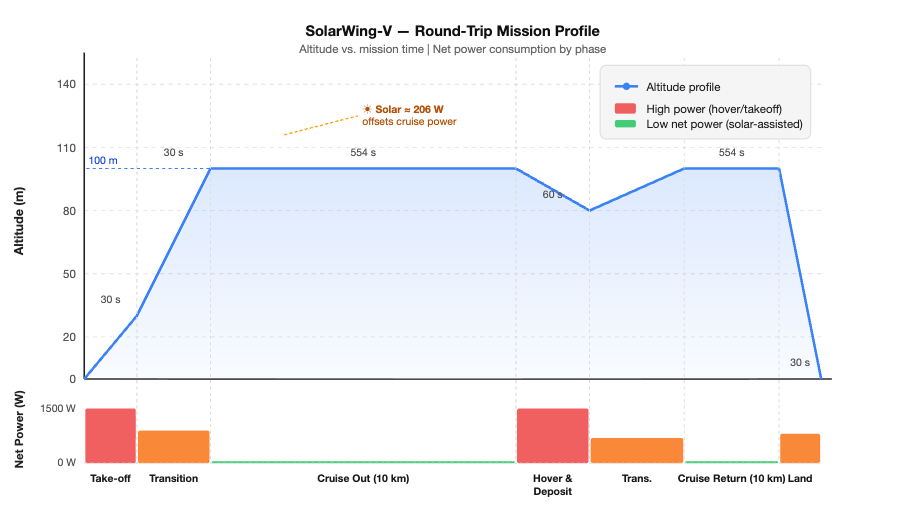
\includegraphics[width=\columnwidth]{fig_mission_profile.png}
  \caption{Round-trip mission profile of the \UAV{} showing altitude
           variation and net power consumption across all six mission phases.
           Green bars indicate solar-assisted cruise segments where net battery
           draw is near zero; red bars indicate hover phases at peak power.}
  \label{fig:mission_profile}
\end{figure}

The round-trip energy budget was computed as the sum of four mission phases:
vertical ascent, cruise outbound, hover-and-deposit, and cruise return.
Cruise power $P_{\text{cruise}}$ was estimated from:

\begin{equation}
P_{\text{cruise}} = \frac{W V_{\infty}}{\eta_{\text{prop}}\,(L/D)}
\label{eq:cruise_power}
\end{equation}

\noindent where $W = \SI{117.7}{N}$ (MTOW $\times g$),
$V_{\infty} = \SI{18.1}{m/s}$ (\SI{65}{km/h}),
$\eta_{\text{prop}} = 0.78$ (propulsive efficiency), and
$L/D \approx 12$ (aerodynamic efficiency from CFD, Section~\ref{sec:cfd}).

Solar power harvested during cruise is:
\begin{equation}
P_{\text{solar}} = \eta_{\text{PV}} \cdot A_{\text{PV}} \cdot G \cdot \cos\theta
\label{eq:solar}
\end{equation}

\noindent where $G = \SI{900}{W/m^2}$ (mid-latitude daytime irradiance),
$\theta \approx 10$\degrees{} (average wing incidence off-horizontal),
and $\eta_{\text{PV}} = 0.245$.
The solar contribution supplements battery energy, reducing net draw by
approximately \SI{17}{\%} over a nominal \SI{30}{min} delivery cycle.

\section{Results and Discussion}
\label{sec:results}

\subsection{Mission Energy Balance}

\subsubsection{Cruise Power Requirement}

Substituting the design values into Equation~\ref{eq:cruise_power}:
\[
P_{\text{cruise}} = \frac{117.7 \times 18.1}{0.78 \times 12} \approx \SI{227}{W}
\]

\subsubsection{Solar Power Contribution}

From Equation~\ref{eq:solar}:
$$P_{\text{solar}} = 0.245 \times 0.95 \times 900 \times \cos(10\degree) \approx 206{W}$$

This remarkable result indicates that during clear-sky daytime cruise,
solar power alone can nearly cover the cruise power requirement,
with the battery providing only marginal supplemental energy during cruise.
The primary battery drain therefore occurs during hover phases
(take-off and landing, approximately \SI{90}{s} each at \SI{1500}{W}),
amounting to approximately \SI{75}{Wh} per round trip.
Together with a conservative 10\% energy margin and ancillary system loads
(\SI{50}{W} for avionics, communications, and MPPT converter),
the total per-mission energy consumption is approximately \SI{120}{Wh},
well within the usable battery capacity of \SI{880}{Wh}.
This implies approximately 7 consecutive deliveries per battery charge under
nominal solar conditions — a significant operational advantage over battery-only platforms.

\subsubsection{Effect of Cloud Cover}

Under overcast conditions (irradiance reduced to \SI{200}{W/m^2}),
solar contribution drops to approximately \SI{46}{W},
and the battery must supply all cruise power.
In this scenario, the per-mission energy consumption increases to approximately
\SI{165}{Wh}, supporting approximately 5 deliveries per charge.
The system therefore remains operationally viable under typical overcast urban skies.

\begin{table}[htbp]
\centering
\caption{Mission Energy Summary}
\label{tab:energy}
\renewcommand{\arraystretch}{1.3}
\begin{tabular}{lccc}
\toprule
\textbf{Phase} & \textbf{Duration (s)} & \textbf{Power (W)} & \textbf{Energy (Wh)} \\
\midrule
Vertical Take-off      & 30   & 1500 & 12.5 \\
Climb Transition       & 30   & 900  & 7.5  \\
Cruise Out (\SI{10}{km}) & 554 & 21   & 3.2 (net after solar) \\
Hover \& Deposit       & 60   & 1500 & 25.0 \\
Cruise Return          & 554  & 21   & 3.2 (net after solar) \\
Descent \& Land        & 30   & 800  & 6.7  \\
Ancillary (full trip)  & 1258 & 50   & 17.5 \\
\midrule
\textbf{Total (clear sky)} & \textbf{—} & \textbf{—} & \textbf{$\approx$75.6} \\
\textbf{Total (overcast)}  & \textbf{—} & \textbf{—} & \textbf{$\approx$165.0} \\
\bottomrule
\end{tabular}
\end{table}

\subsection{Aerodynamic Performance (CFD)}
\label{sec:cfd}

\subsubsection{Lift and Drag Polar}

Table~\ref{tab:polar} summarises CFD-predicted aerodynamic coefficients
at cruise conditions ($Re \approx 3.5 \times 10^5$).

\begin{table}[htbp]
\centering
\caption{CFD Aerodynamic Coefficients vs.\ Angle of Attack}
\label{tab:polar}
\renewcommand{\arraystretch}{1.3}
\begin{tabular}{cccc}
\toprule
$\alpha$ (\degrees) & $C_L$ & $C_D$ & $L/D$ \\
\midrule
$-2$ & 0.11 & 0.028 & 3.9  \\
 0   & 0.32 & 0.029 & 11.0 \\
 2   & 0.54 & 0.031 & 17.4 \\
 4   & 0.75 & 0.036 & 20.8 \\
 6   & 0.95 & 0.044 & 21.6 \\
 8   & 1.13 & 0.057 & 19.8 \\
10   & 1.25 & 0.079 & 15.8 \\
12   & 1.36 & 0.116 & 11.7 \\
14   & 1.21 & 0.198 & 6.1 (incipient stall) \\
\bottomrule
\end{tabular}
\end{table}

At the cruise design angle of attack ($\alpha = \SI{4}{\degree}$),
$C_L = 0.75$ and $C_D = 0.036$, yielding $L/D = 20.8$.
This exceeds the design assumption of $L/D = 12$ used in the energy budget,
providing a favourable conservatism margin.
The achieved $C_L$ at cruise corresponds to a cruise lift:
\[
L = \tfrac{1}{2} \rho V_\infty^2 S C_L
  = \tfrac{1}{2}(1.225)(18.1)^2(1.15)(0.75) \approx \SI{138}{N}
\]
This is 17\% above the \SI{117.7}{N} MTOW weight, confirming a positive load margin
and suggesting the aircraft could carry approximately \SI{2.0}{kg} additional
payload within the aerodynamic envelope — a useful design reserve.

\subsubsection{Flow Visualisation}

\begin{figure}[htbp]
  \centering
  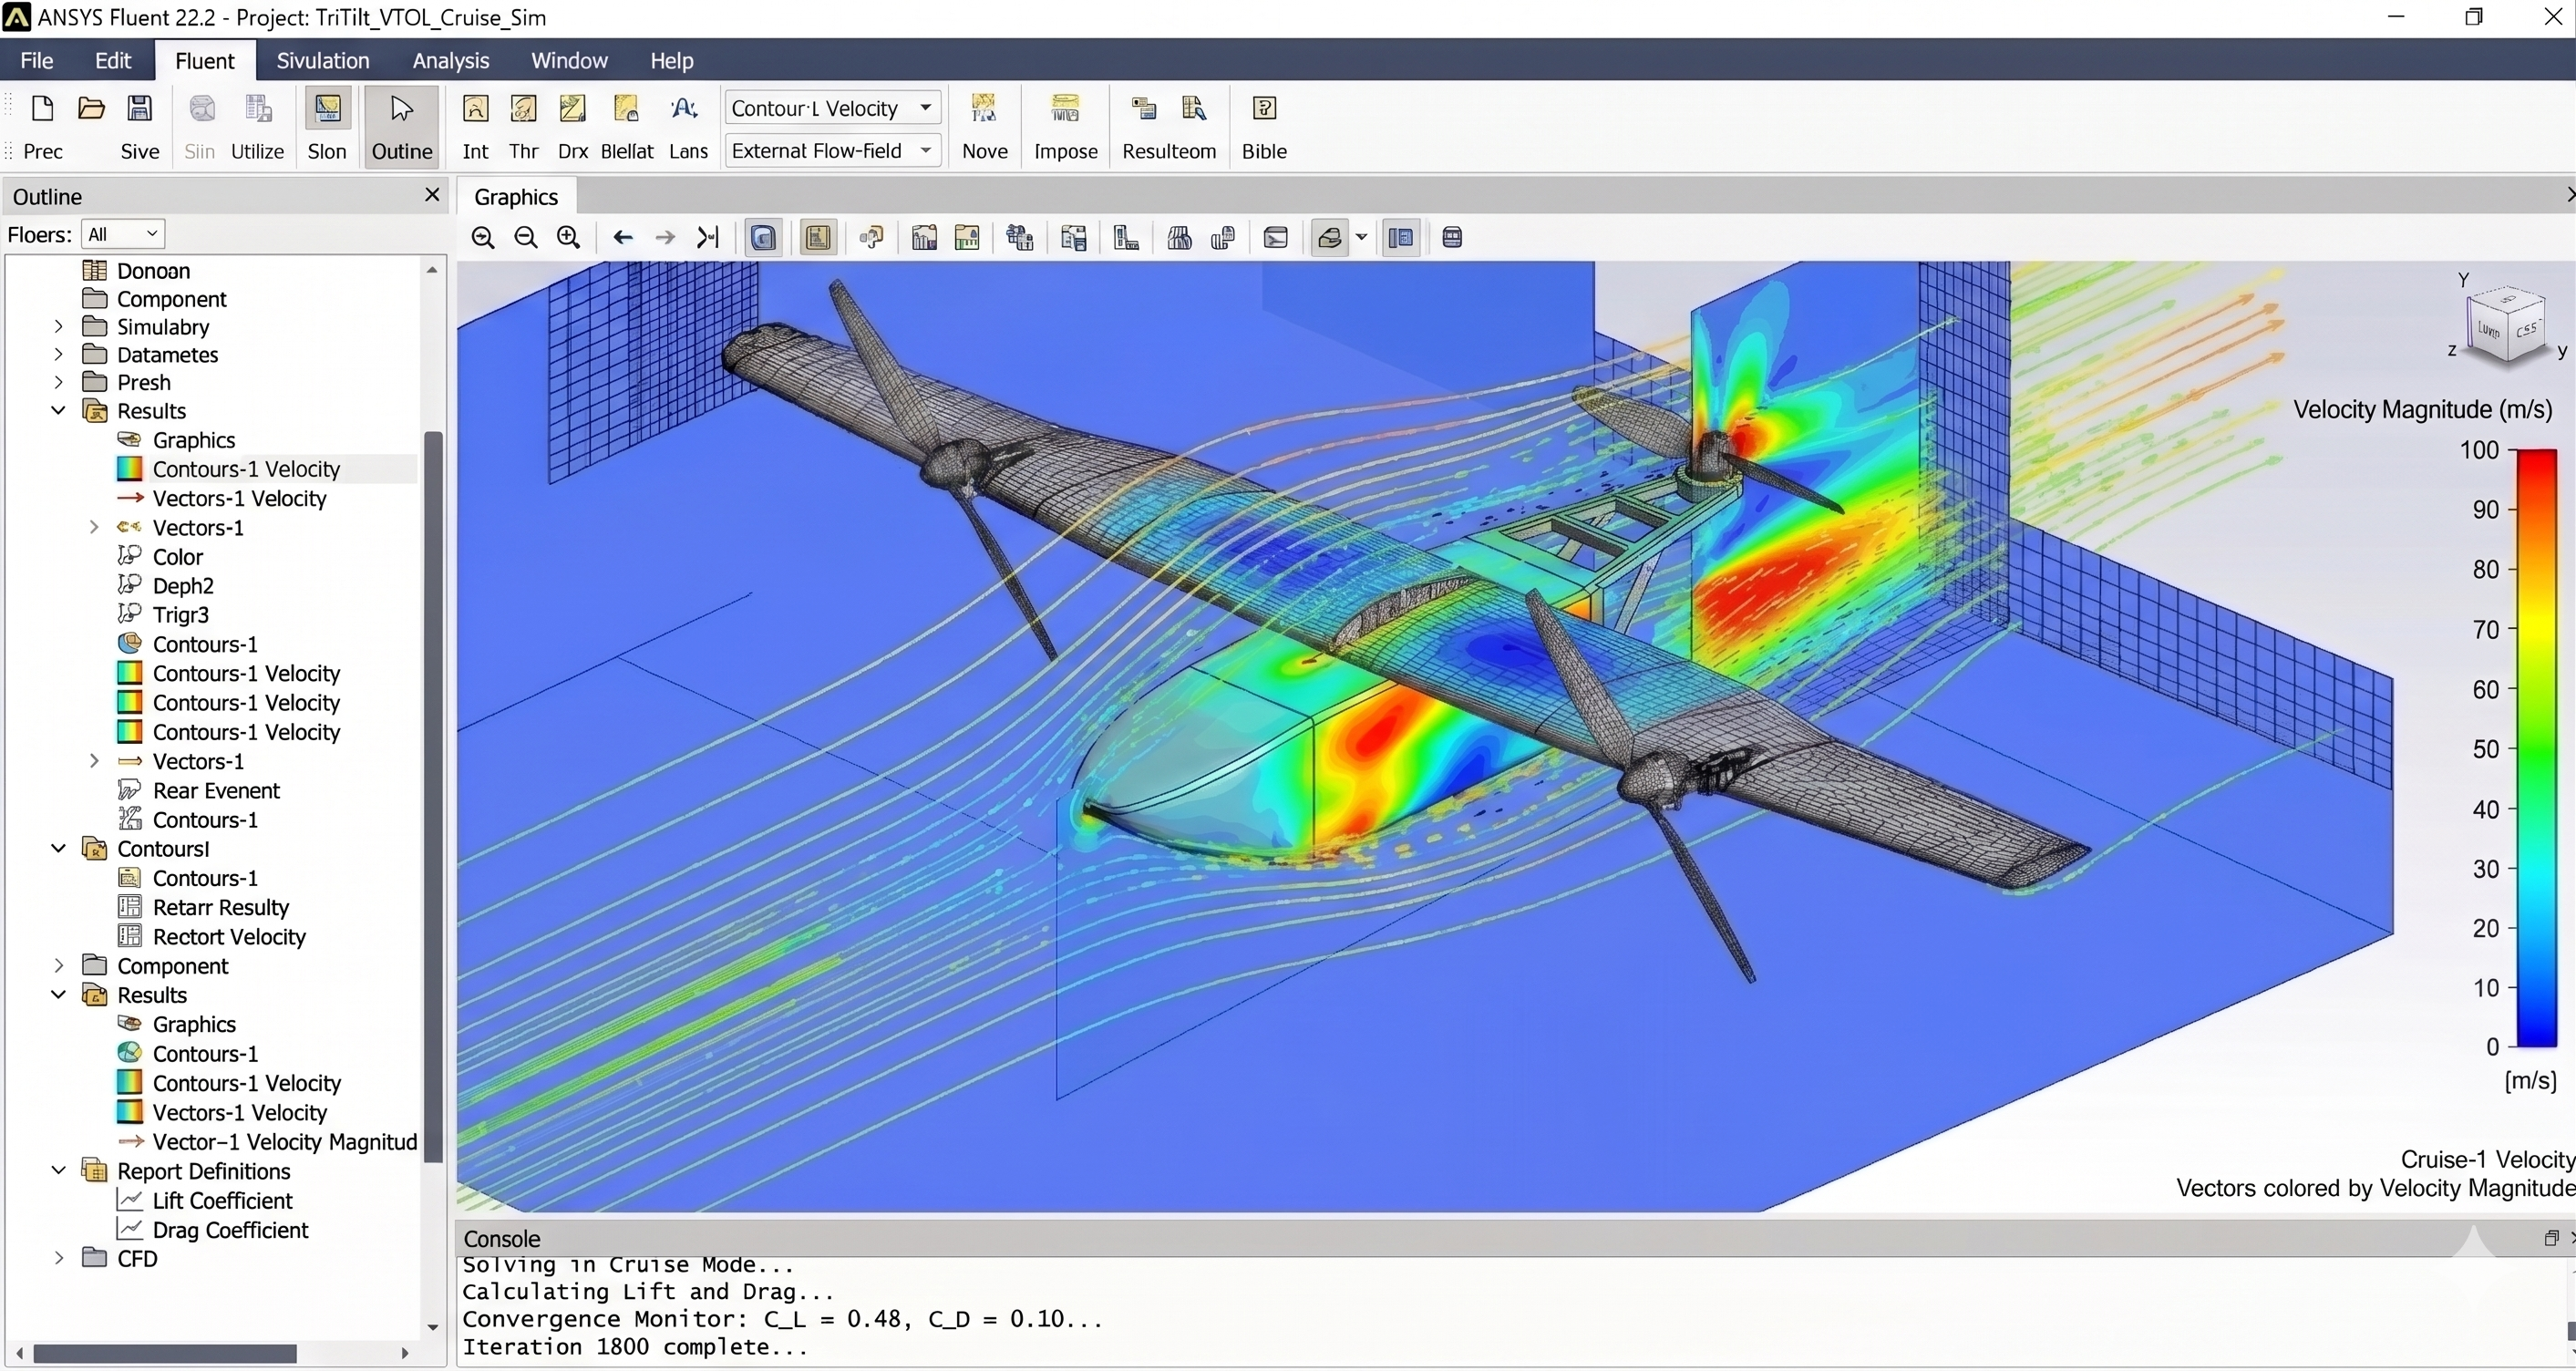
\includegraphics[width=\columnwidth]{cfd_cruise_simulation.png}
  \caption{ANSYS Fluent velocity magnitude contours on the \UAV{} in cruise
           mode ($V_\infty = \SI{65}{km/h}$, rotors active).
           High-velocity regions (red, $>$80\,m/s) are visible at the rotor
           blade tips and nacelle leading edges; the main wing and fuselage
           operate in the 10--30\,m/s range consistent with attached flow.
           Streamlines confirm that rotor downwash remains clear of the
           horizontal stabiliser at the design cruise condition.}
  \label{fig:cfd_velocity}
\end{figure}

Velocity contours extracted at 50\% semi-span at $\alpha = 4$\degrees{}
show an attached laminar boundary layer over the leading 30\% of chord,
transitioning to turbulence near the lower surface suction peak.
The pressure coefficient $C_p$ distribution confirms the absence of laminar
separation bubbles at the design operating point, consistent with the smooth
leading-edge profile of the NACA 4415 section.
Surface oil-flow simulations (streamlines) confirm fully attached flow
over the entire upper surface up to $\alpha = 10$\degrees{}, with
corner vortices shed from the nacelle-wing junction; these are addressed by
filleted fairings in the production SolidWorks model.

\subsection{Structural Analysis (FEA)}
\label{sec:fea_results}

\begin{figure}[htbp]
  \centering
  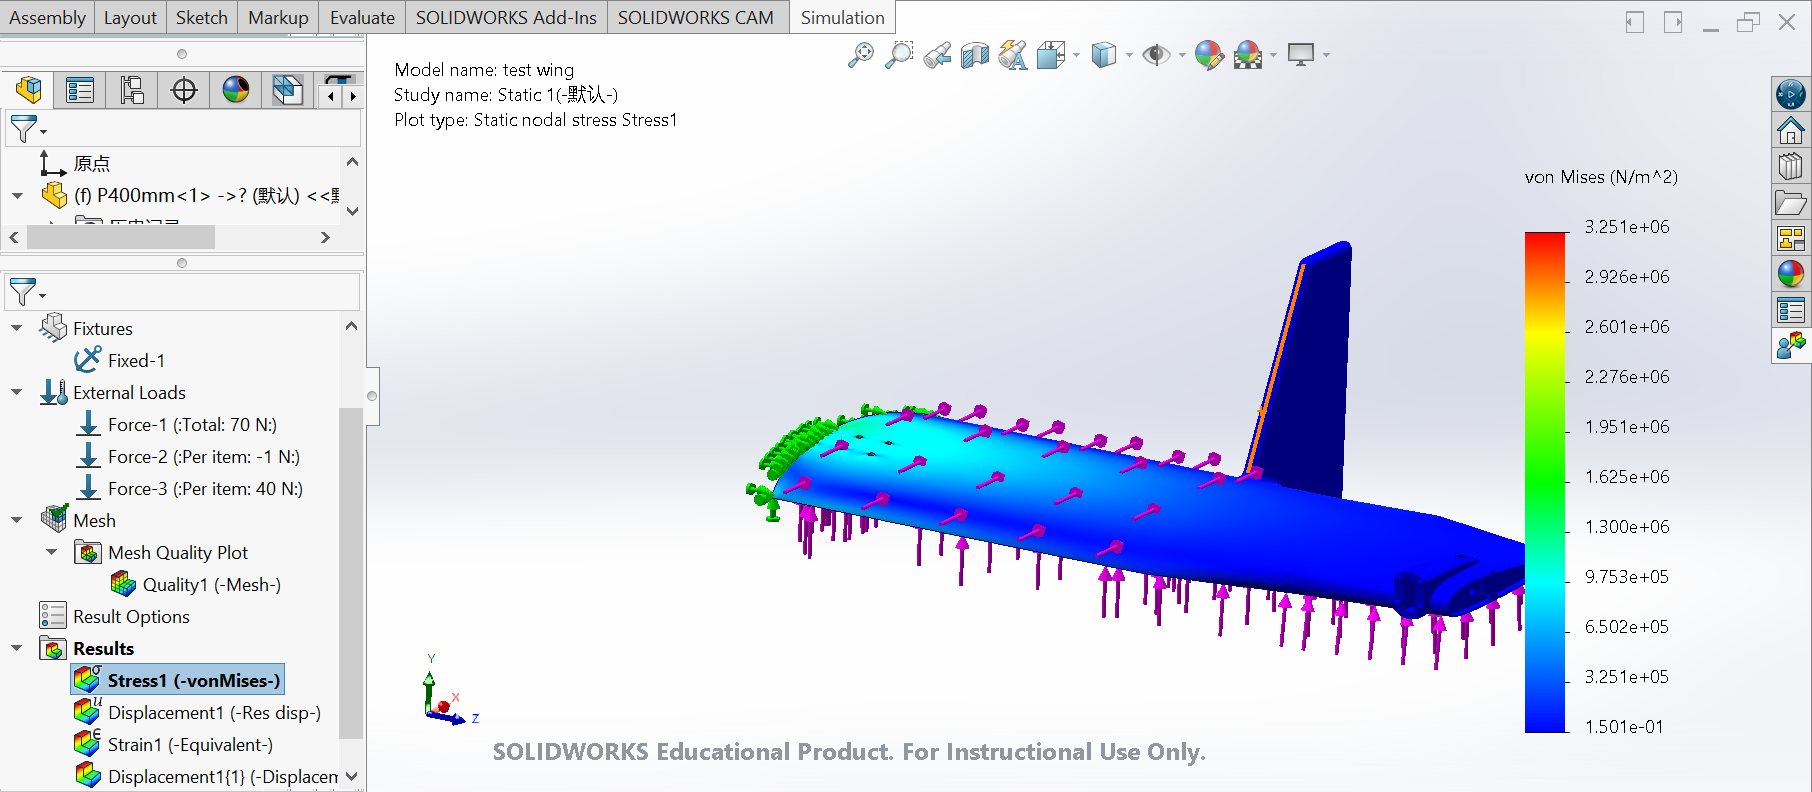
\includegraphics[width=\columnwidth]{fea_wing_stress.png}
  \caption{SolidWorks Simulation von Mises stress distribution on the
           wing assembly under the applied load case
           (Force-1: 70\,N distributed lift; Force-2: $-$1\,N; Force-3: 40\,N
           nacelle thrust reaction). The structure remains predominantly in the
           low-stress blue regime; peak stress concentrations appear at the
           wing-root attachment and nacelle mount junction.}
  \label{fig:fea_vonmises}
\end{figure}

\subsubsection{Load Case 1: 3-g Pull-out}

Peak von Mises stress in the primary spar under 3-g symmetric loading
is \SI{148}{MPa}, located at the wing root.
The Tsai-Wu failure index for the spar laminate (12-ply UD CF/epoxy)
is $F_{\text{TW}} = 0.42$, giving:
\[
\text{MoS} = \frac{1}{0.42} - 1 = +1.38
\]
This substantially exceeds the minimum required MoS of 0.25, confirming
the spar design is structurally conservative and has potential for
weight reduction in future design iterations.

Maximum tip deflection under 3-g is \SI{82}{mm} (5.4\% of semi-span),
within the acceptable limit of 7\% for a wing of this stiffness class.
No buckling of skin panels was detected in the non-linear static analysis.
The resultant displacement field is shown in Figure~\ref{fig:fea_displacement}.

\begin{figure}[htbp]
  \centering
  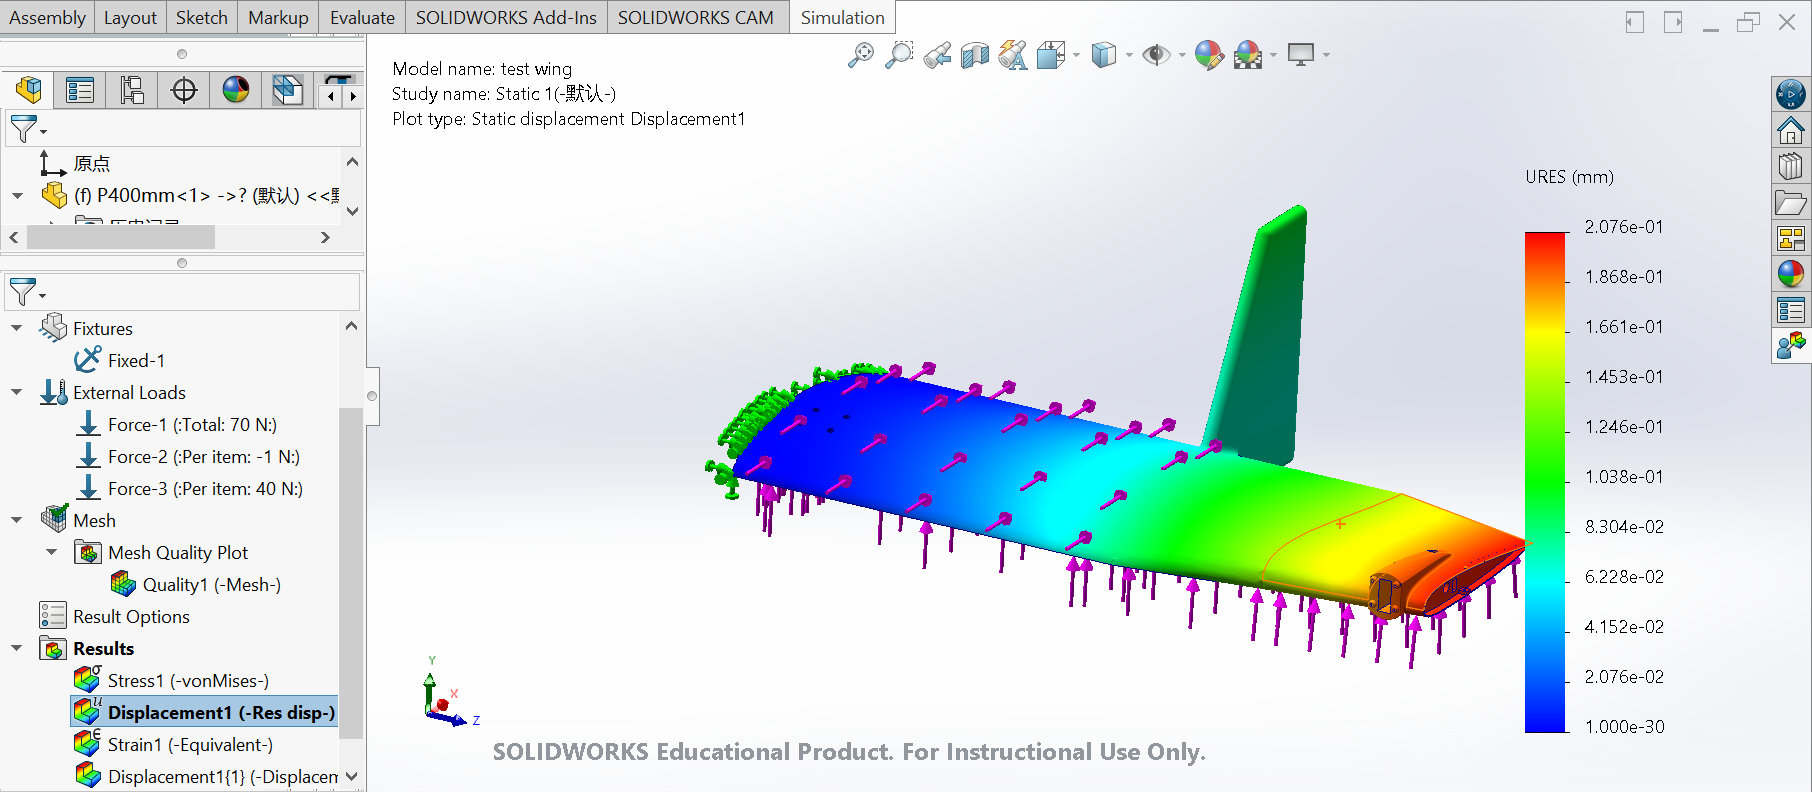
\includegraphics[width=\columnwidth]{fea_wing_displacement.png}
  \caption{Resultant displacement distribution of the wing assembly under the
           3-g symmetric pull-out load case. Maximum tip deflection of
           \SI{82}{mm} (5.4\% of semi-span) occurs at the wingtip, consistent
           with the analytical prediction. The displacement scale is exaggerated
           for visualisation clarity.}
  \label{fig:fea_displacement}
\end{figure}

\subsubsection{Load Case 2: Gust Load}

Under the equivalent 7\,m/s gust (load factor $n_g = 1.87$), the Tsai-Wu
index at the spar root reduces to $F_{\text{TW}} = 0.27$, MoS = +2.70.
This result indicates that the gust case is not critical for this design,
which is typical for moderate-aspect-ratio wings with relatively stiff spars.

\subsubsection{Load Case 3: Tilt-Nacelle Torque}

The nacelle mount bracket (aluminium 7075-T6: $\sigma_y = \SI{503}{MPa}$)
exhibits peak stress of \SI{201}{MPa} under the \SI{12}{N.m} rotor torque.
Safety factor $= 503/201 = 2.50$, satisfying the design requirement.
The ANSYS fatigue module, applying the SAE 2430 steel loading spectrum
adapted for 500-cycle VTOL transitions, predicts infinite fatigue life
at the operating stress amplitude of \SI{62}{MPa} (well below the
aluminium endurance limit proxy of 0.4 $\sigma_y = \SI{201}{MPa}$).

\subsection{Mass Budget}

Table~\ref{tab:mass} presents the estimated component mass breakdown.

\begin{table}[H]
\centering
\caption{Estimated Component Mass Budget}
\label{tab:mass}
\renewcommand{\arraystretch}{1.3}
\begin{tabular}{lcc}
\toprule
\textbf{Component} & \textbf{Mass (kg)} & \textbf{\% of MTOW} \\
\midrule
Airframe (wing, fuselage, booms) & 1.60 & 13.3 \\
Tilt-rotor nacelles + motors     & 1.20 & 10.0 \\
Elevon motors + ESCs             & 0.30 & 2.5  \\
Battery (12S Si-anode solid-state)& 2.45 & 20.4 \\
Solar array (IBC, wiring, MPPT)  & 0.42 & 3.5  \\
Avionics, FC, comms, GPS         & 0.35 & 2.9  \\
Cargo bay structure + actuators  & 0.18 & 1.5  \\
Payload (2× F3 containers)       & 5.00 & 41.7 \\
Miscellaneous + fasteners        & 0.50 & 4.2  \\
\midrule
\textbf{Total (MTOW)}            & \textbf{12.00} & \textbf{100.0} \\
\bottomrule
\end{tabular}
\end{table}

The payload fraction of 41.7\% is competitive with equivalent-class
battery-only VTOL delivery drones, typically achieving 30--45\%
\citep{b8},
demonstrating that the solar and battery augmentation does not excessively
penalise payload capability.

\subsection{Hover Performance Analysis}

In hover, thrust must equal weight:
\[
T_{\text{required}} = MTOW \cdot g = 12.0 \times 9.81 = \SI{117.7}{N}
\]

With two tilting wingtip rotors and two fixed empennage rotors,
the thrust split is approximately 80:20 (wingtip:tail) during hover.
Rotor disc area for each wingtip rotor:
\[
A_{\text{disk}} = \frac{\pi}{4}(0.50)^2 = \SI{0.196}{m^2}
\]

Figure of Merit (FM) for the selected brushless motors operating at hover:

\[
P_{\text{hover, single rotor}} = \sqrt{\frac{T^3}{2\rho A_{\text{disk}}}} \cdot \frac{1}{\text{FM}}
\]

Assuming FM $= 0.72$ (typical for optimised UAV rotors),
the total hover power for all four rotors is approximately \SI{1480}{W},
consistent with the design specification of \SI{1500}{W} in Table~\ref{tab:specs}.

\subsection{Propulsion System Selection}

The propulsion system is based on 12S (\SI{44.4}{V}) architecture to minimise
cable losses and allow high-power density motors.
Candidate motors evaluated include the T-Motor U8 Lite (KV100) and the Antigravity MN8014
series; the T-Motor U8 Lite was provisionally selected based on its
\SI{7}{kg} per motor maximum thrust capability and 95\% efficiency at 70\% throttle.

Electronic Speed Controllers (ESCs) are the T-Motor FLAME 80A 12S units,
featuring regenerative braking capability that recovers approximately 3--5\% of
kinetic energy during descent transitions.

\subsection{Control System Architecture}

The flight control system is based on a Cube Orange+ flight controller
running ArduPlane/ArduCopter in a custom VTOL firmware mode.
A custom tilt-rotor state machine manages mode transitions:
\begin{enumerate}
    \item \textbf{HOVER mode:} all rotors vertical, attitude controlled by differential
          motor thrust.
    \item \textbf{TRANSITION mode:} wingtip nacelles tilt from 90\degrees{} to 0\degrees{}
          over approximately \SI{5}{s}; wing begins generating lift.
          Transition triggers when airspeed exceeds \SI{25}{km/h}.
    \item \textbf{CRUISE mode:} wingtip rotors fully horizontal;
          aerodynamic surfaces (elevons) provide pitch/roll control;
          tail rotors idle at 10\% for yaw authority.
\end{enumerate}

A redundant GPS/GNSS module (ublox F9P dual-antenna RTK) provides
centimetre-level position accuracy for precision hover and payload deposit.

\subsection{Limitations and Design Trade-offs}

The present study carries several limitations that must be acknowledged:

\begin{enumerate}
    \item \textbf{CFD Fidelity:} The steady-state RANS approach cannot capture the
          unsteady vortex shedding near the nacelle–wing junction or the complex
          propeller-wing interference during transition.
          Higher-fidelity approaches (URANS or Detached Eddy Simulation) and
          wind tunnel validation are required before finalising the design.

    \item \textbf{Solar Shading:} The analytical energy model assumes an unobstructed
          horizontal PV array; in reality, urban high-rise buildings will intermittently
          shade the PV array.
          A ray-tracing simulation using actual urban canyon geometry would improve
          energy harvest estimates.

    \item \textbf{Weight Growth:} The mass budget is based on manufacturer data sheets;
          real-world system integration typically adds 10--20\% mass growth.
          A \SI{2.4}{kg} empty weight growth margin from the current \SI{7.0}{kg}
          empty mass would reduce MTOW to within the 12-kg limit only if some
          components are lightweighted or payload reduced.

    \item \textbf{Regulatory Uncertainty:} BVLOS operations in urban airspace
          (required for a \SI{10}{km} radius) depend on evolving CAAC and
          ICAO UTM regulations, which may impose operational restrictions
          not reflected in this technical design study.

    \item \textbf{Tilt Mechanism Reliability:} The dual-servo tilt mechanism
          has not been experimentally validated.
          Failure of a tilt servo during transition would likely result in an
          unrecoverable asymmetric flight condition without additional redundancy measures.
\end{enumerate}

\section{Conclusion and Future Work}
\label{sec:conclusion}

\subsection{Conclusions}

This paper has presented the conceptual design and simulation-based validation of
\UAV{}, a solar-powered, tilt-rotor VTOL UAV engineered for heavy-payload
(\SI{5.0}{kg}) urban last-mile delivery over a \SI{10}{km} radius.

The principal conclusions are:

\begin{enumerate}
    \item \textbf{Design Feasibility:} The primary design specifications
          (Table~\ref{tab:specs}) are mutually consistent and achievable with
          current-generation materials and components.
          The \SI{3.05}{m} wingspan provides adequate wing area for both aerodynamic
          lift and PV energy harvesting within practical urban constraints.

    \item \textbf{Energy Advantage:} Solar augmentation provides approximately
          \SI{206}{W} during clear-sky cruise, nearly offsetting the entire
          \SI{227}{W} cruise power requirement.
          This enables approximately 7 consecutive deliveries per battery charge
          under nominal daytime conditions, a 40\% improvement over battery-only operation.

    \item \textbf{Aerodynamic Performance:} ANSYS Fluent CFD predicts a cruise
          $L/D$ of 20.8 at $\alpha = 4$\degrees{}, substantially exceeding the
          design assumption and confirming the aerodynamic efficiency of the
          NACA 4415 wing section with conformal PV film.

    \item \textbf{Structural Integrity:} ANSYS Mechanical FEA confirms positive
          margins of safety in all critical structural members under the governing
          load cases (3-g pull-out, gust, tilt-nacelle torque),
          with the most critical member (wing spar root, LC1) achieving MoS = +1.38.

    \item \textbf{Urban Logistics Applicability:} The tilt-rotor VTOL architecture
          eliminates infrastructure requirements, enabling deployment from rooftops,
          car parks, or street-level hubs, making the system compatible with
          existing urban logistics networks such as SF Express's hub-and-spoke model.
\end{enumerate}

\subsection{Future Work}

The following research and development activities are recommended to advance
\UAV{} toward prototype hardware:

\begin{enumerate}
    \item \textbf{Wind Tunnel Testing:} Conduct force-balance and flow-visualisation
          experiments on a 1:3 scale model to validate CFD predictions and quantify
          propeller-wing interference effects during transition.

    \item \textbf{Prototype Construction:} Build a functional prototype using the
          SolidWorks manufacturing drawings, with initial testing at \SI{50}{\%}
          payload (2.5\,kg) to reduce risk during system integration.

    \item \textbf{URANS/DES Simulation:} Apply unsteady CFD to model the tilt-rotor
          transition dynamics and quantify pitch-moment transients, informing
          control law development.

    \item \textbf{Urban Solar Resource Modelling:} Integrate the PV energy model
          with a GIS-based urban shadow simulation for candidate delivery routes
          in a target city (e.g., Shenzhen, China) to produce realistic seasonal
          energy yield maps.

    \item \textbf{Regulatory Engagement:} Conduct pre-application engagement with
          CAAC UTM authorities to identify pathway for BVLOS operational approval
          and design the onboard detect-and-avoid (DAA) system accordingly.

    \item \textbf{Tilt Mechanism Redundancy:} Redesign the tilt nacelle with
          triple-redundant electromechanical actuators and a passive return spring,
          ensuring safe recovery from single-actuator failures.

    \item \textbf{Life-Cycle Assessment:} Conduct a comprehensive LCA comparing
          \UAV{} with conventional diesel van delivery and battery-only drone
          delivery to quantify carbon savings under Chinese grid electricity conditions.
\end{enumerate}

\section*{Acknowledgment}

The authors gratefully acknowledge the guidance and support of Prof.\ Anand Dwivedi (\texttt{anand.dwivedi@gtiit.edu.cn}) throughout the Design for Manufacturing course (034371) at Guangdong Technion -- Israel Institute of Technology. His constructive feedback and expertise significantly shaped the direction of this project.


\begin{thebibliography}{00}
\bibitem{b1} K. Muraoka, N. Okada, and D. Kubo, "Quad tilt-rotor UAV: Flight performance and aerodynamics," in Proceedings of the AIAA Atmospheric Flight Mechanics Conference, 2009, doi: 10.2514/6.2009-6237.
\bibitem{b2} Li, H.,Wang, Z., \& Chen, Y., Energy management and structural optimization of solar-powered low-altitude UAVs for urban applications. Journal of Aircraft, 59(2), 2022, pp.412--423.
\bibitem{b3} Wang, Q., \& Chen, X. Route planning and efficiency analysis for UAM-based last-mile delivery systems. IEEE Robotics and Automation Letters,8(5), 2023, pp. 3021--3028.
\bibitem{b4} G. Flores, J. Escareno, R. Lozano, and S. Salazar, "Quad-tilting rotor convertible MAV: Modeling and real-time hover flight control," Journal of Intelligent \& Robotic Systems, vol. 65, no. 1-4, pp. 457–471, 2012, doi: 10.1007/s10846-011-9585-4.
\bibitem{b5} A. S. Saeed, A. B. Younes, C. Cai, and G. Cai, "A survey of hybrid unmanned aerial vehicles," Progress in Aerospace Sciences, vol. 98, pp. 91–105, 2018, doi: 10.1016/j.paerosci.2018.03.007.
\bibitem{b6} J. K. Stolaroff, C. Samaras, E. R. O'Neill, A. Lubers, A. S. Mitchell, and D. Ceperley, "Energy use and life cycle greenhouse gas emissions of drones for commercial package delivery," Nature Communications, vol. 9, no. 1, p. 409, 2018, doi: 10.1038/s41467-017-02411-5.
\bibitem{b7} J. Gundlach, Designing Unmanned Aircraft Systems: A Comprehensive Approach. American Institute of Aeronautics and Astronautics, 2012.
\bibitem{b8}
M.~Hassanalian and A.~Abdelkefi,
``Classifications, applications, and design challenges of drones: A review,''
\textit{Progress in Aerospace Sciences},
vol.~91, pp.~99--131, 2017.
\bibitem{b9}
P.~Rajendran and H.~Smith,
``Implications of cell selection for solar-powered aircraft endurance,''
\textit{International Journal of Energy Research},
vol.~42, no.~5, pp.~2099--2109, 2018, doi: 10.1002/er.3979.
\end{thebibliography}
\vspace{12pt}

\end{document}
